\documentclass{princeton_astro_thesis}
\RequirePackage[T1]{fontenc}
\RequirePackage[margin=1in,inner=1.5in]{geometry}
\RequirePackage{setspace}
\doublespacing
%\linespread{2}
\usepackage{amsmath}
\usepackage{graphicx}
\usepackage[utf8]{inputenc}
\usepackage{caption,subcaption}
\graphicspath{ {/Users/Teva/Senior-Thesis} }
%these can be specified in your .cls file if you want the main.tex file to look cleaner
\author{Teva Ilan}
\title{Insert Title}
\abstract{When Cosmic Microwave Background (CMB) photons interact with free electrons in the hot gas of galaxy clusters they gain energy via inverse Compton scattering, resulting in a spectral distortion of the CMB called the Sunyaev--Zel'dovich (SZ) effect. This phenomena is invaluable to cosmology as it facilitates measurements of various properties of galaxy clusters and cosmological parameters. In this work, we use CMB maps from the Atacama Cosmology Telescope (ACT) the Planck satellite and the redMaPPer galaxy cluster catalog to fit for the thermal SZ (tSZ effect), the kinetic SZ (kSZ effect), the dust, and the relativistic SZ (rSZ) effect. Though we do not detect kSZ or rSZ using an mcmc fitting algorithm, we are able to put constraints on both of these quantities. }

\adviser{Your Advisor}
\date{Star Wars Day}
%begin thesis content
\begin{document}
\chapter{Introduction}
\section{Background}

%Understanding the relationship between between the amount of gas in galaxy clusters and the number of galaxies in the cluster (i.e. the richness of the cluster) is important for a few reasons. First of all, it informs the astrophysics of galaxy cluster formation. Because non-gravitational processes, such as AGN feedback and supernovae are thought to play a role in galaxy and galaxy group formation, we expect that they will cause deviations from the richness-gas relation that we would get if only gravitational processes were involved. Thus learning about the richness-gas scaling relation can tell us how more about how non-gravitational processes are involved in galaxy and galaxy group formation. 
%\par Secondly as both richness and an effect of the gas called the SZ effect are used as ways of finding clusters and as proxies for their mass it is important to understand how they are related. The SZ effect is the result of inverse Compton scattering of photons from the CMB off of high energy electrons in hot gas. When CMB photons go through hot cluster gas they gain energy from the high energy electrons. Then when we measure the CMB these photons produce a frequency-dependent change in the observed CMB temperature along the Line-of-Sight to the galaxy cluster. 
%\par In order to determine the relationship between the richness of clusters and the amount of gas in them we used CMB maps from ACT and the redMaPPer galaxy group catalog. The 1.4 arcminute resolution of ACT gives its CMB maps a higher resolution than those made with the Planck satellite. The ACT CMB maps we used in our analysis were taken at 250 GHz. We used the redMaPPer catalog because it contains good measurements of cluster richness and many of the cluster were located within our CMB maps. RedMaPPer is a red-sequence cluster finder, which means that it finds galaxy cluster candidates by looking for over densities of galaxies that form a red sequence.
\par The Sunyaev--Zel'dovich (SZ) effect results from inverse Compton scattering of CMB photons off of the hot gas in galaxy clusters. The dominant component of this effect results from interactions between Cosmic Microwave Background (CMB) photons and electrons in the gas that have high energies as a result of their temperature. This produces a frequency dependent shift in the observed CMB temperature along the Line-of-Sight (LOS) to the galaxy cluster and is known as the thermal SZ (tSZ) effect (Greco et al.). The shape of the distortion of the observed CMB due to the tSZ effect is constant to first order but there is a higher order dependency on the temperature of the gas due to relativistic corrections. This is called the relativistic SZ effect (rSZ) (Hincks et al, 2018). There is also a second order effect that results from interactions between the CMB photons and electrons in the gas that have high energies as a result of their bulk motion. This effect depends on the peculiar velocity of the cluster, has no frequency dependence, and is known as the kinetic SZ (kSZ) effect (Hincks et al., 2018). The relativistic corrections to the kSZ effect are far below current sensitivities (Erler, 2018). 
%\par Defining the dimensionless frequency as $x\equiv h\nu_i/2k_B T_{CMB}$, we can write the SZ effect as an intensity shift relative to the CMB,
%\begin{equation}
%\frac{\Delta I_{SZ}}{I_0}=h(x)\left[f(x,T_{eff})y-\tau_{e}\left(\frac{v_{pec}}{c}\right)\right],
%\end{equation}
%where $I_0=2(k_B T_{CMB})^3/(hc)^2$, $h(x)=x^4 e^x/(e^x-1)^2$, y is the Compton y-parameter which is a measure of the electron pressure integrated along the LOS, $\tau_e$ is the optical depth of the plasma, and $v_pec$ is the LOS peculiar velocity in the rest frame of the CMB.
\par Thus the tSZ effect can be used as a proxy for the mass of or the amount of gas in clusters, the kSZ effect can be used to measure the peculiar velocity of clusters, and the rSZ effect can be used to measure the gas temperature. Understanding the tSZ signal and thus understanding the amount of gas in clusters is important because it informs the astrophysics of galaxy cluster formation. The kSZ effect is the only method of directly measuring peculiar velocities at cosmological distances. Using kSZ to measure the peculiar velocities of individual clusters requires models of the intracluster medium (De Bernardis et al., 2017). However, such models are not required to constrain bulk kSZ. The kSZ effect is important as a measurement of bulk kSZ which can be used to constrain radial inhomogeneity in the peculiar velocities of galaxy clusters. An alternative explanation for the apparent accelerating expansion of the universe due to dark energy is that our galaxy is located in a giant under-dense void and the observed acceleration is due to the peculiar velocities of galaxy clusters rather than a change in the rate of cosmic expansion (Bull et al., 2012). One of the goals of this work was to put a constraint on bulk kSZ, which is important given the fact that our understanding of cosmology is based on homogeneity on large scales. A detection of bulk kSZ would derail this foundational assumption of cosmology.
\par Trying to measure rSZ is important because if measurable, it would provide an additional means of measuring the gas temperature in clusters, which is traditionally done via X-ray spectroscopy (Hincks et al, 2018). Though rSZ is a higher order effect it can be on the order of a few percent at certain frequencies and ignoring it can lead to an underestimation of the Compton-y parameter. This in turn results in a biased Y--M relation, which is used to estimate cosmological parameters (Hincks et al, 2018). Additionally, apart from a recent claimed detection by Hincks et al., rSZ has never been detected. Thus, constraining or detecting rSZ is itself a topic of interest. In this work, we were able to constrain rSZ but failed to make a detection with the available data. 
\par Past research has constrained bulk kSZ. For example, in 2014 the Planck collaboration used the Planck data and the Meta Catalogue of X-ray detected Clusters of galaxies to put an upper limit of  $254\, km/s$ (95\% confidence level) on bulk flow. These results were consistent with $\Lambda CDM$ cosmology and combined with supernova observations were able to rule out many inhomogeneous void models that were proposed as alternatives to dark energy (Planck, 2014). However, the catalog and maps we use have not previously been utilized to put a constraint on bulk kSZ. 
\par As mentioned earlier, there has only been one claimed detection of rSZ. This detection by Hincks et al. was at the $5\sigma$ level and was accomplished using the Planck DR2 maps at 5 different frequencies (70, 100,
143, 217 and 353 GHz) and 47 galaxy clusters they selected from the Planck SZ1 cluster catalogue. In analyzing this data they used an affine invariant Markov chain Monte Carlo (MCMC) sampler implemented via the emcee python package to obtain the best fit parameters (Hincks et al, 2018). Though our fitting methodology is similar to Hincks et al., the data we use is different and has not previously been applied to constrain or detect rSZ.
\par This work is structured as follows: Section 2 provides a description of the data (maps and catalogs) that we used in our analysis. Section 3 our methodology for analyzing this data and fitting for the quantities of interest as well as some of the theory behind this methodology. In Section 4, we present the results of our data analysis. These results are then discussed in Section 5. Section 6 provides an overview of possible areas for future research. 


\chapter{Data}
\section{CMB Maps}
We used CMB maps at 5 frequencies: 90 GHz, 150 GHz, 217 GHz, 353 GHz, 545 GHz, and 857 GHz. The 90 GHz and 150 GHz maps are from the Atacama Cosmology Telescope (ACT) while the high frequency maps are from the Planck satellite. All of the maps go from -44 degrees to 46 degrees in right ascension and -9 degrees to 5 degrees in declination. Using maps from multiple frequencies allows us to disentangle different components of the observed flux from each other, specifically the dust component, the tSZ effect component, the kSZ effect component, and the rSZ effect component. It should also be noted that the ACT maps that we refer to as the  90 GHz and 150 GHz maps actually combine data from multiple frequencies. The "90 GHz" ACT map is a coadd of Planck 100 GHz and all ACTPol 90 GHz night-time data collected from 2013-2015. Similarly, the "150 GHz" ACT map is a coadd of Planck 143 GHz and all ACTPol 150 GHz night-time data collected during the same time period.
\section{Galaxy Cluster Catalogs}
Our work involved two sets of galaxy cluster catalogues: the redMaPPer and an ACT confirmed cluster catalog. RedMaPPer is a red-sequence cluster finder, which means that it finds galaxy cluster candidates by looking for over densities of galaxies that form a red sequence. Our main analysis only uses the redMaPPer catalog. Of the 2198 galaxy clusters in the redMaPPer catalog, over 14,000 were located on the maps we used and sufficiently far from point sources to be used in our analysis. Some properties of the redMaPPer catalog are shown in the two plots below.
\begin{figure}[h]
\centering
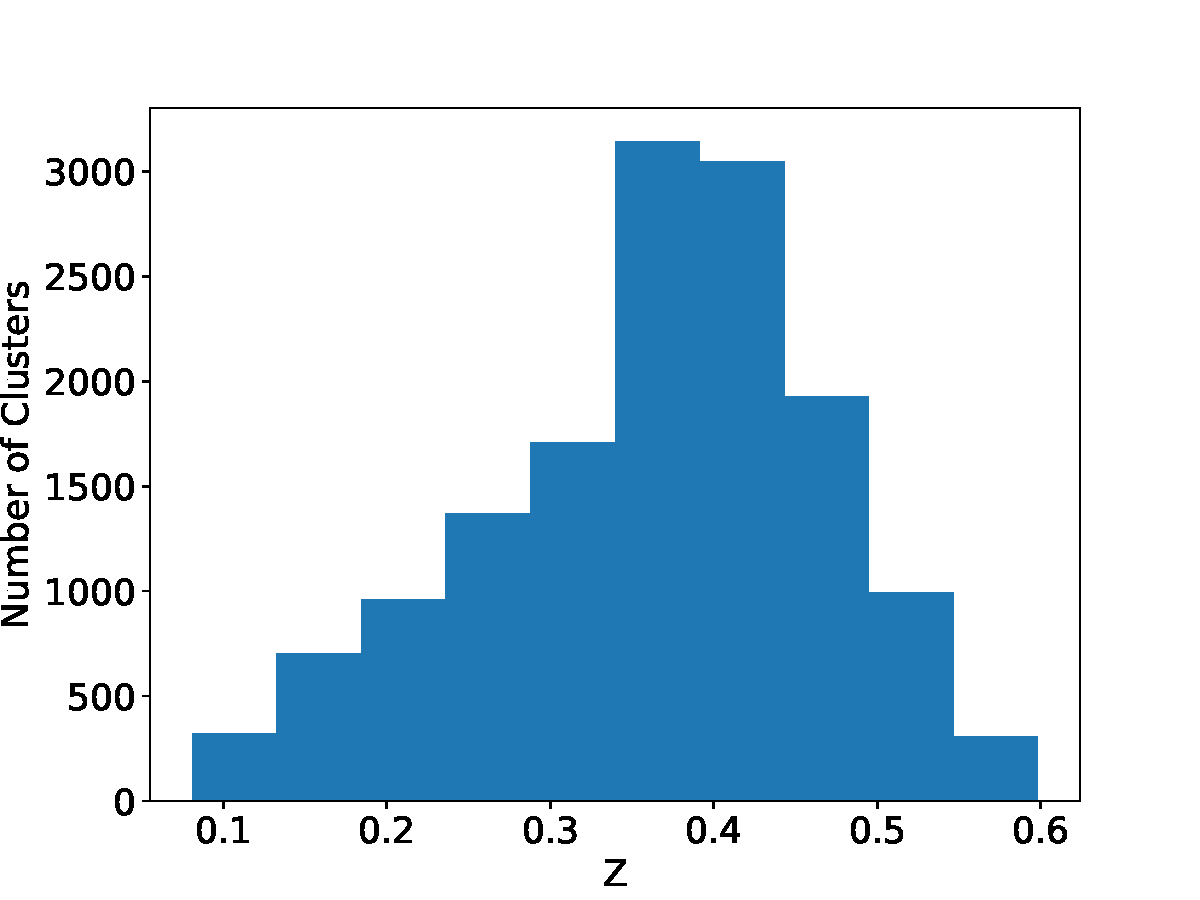
\includegraphics[width=0.5\textwidth]{../redmapper_z_hist.pdf}
\caption{This plot shows a histogram of the distribution of redshifts of the clusters in the RedMaPPer catalog. Evidently, the clusters in the RedMaPPer catalog range from $z\approx0.05$ to $z\approx0.6$. Note that this plot only includes clusters from RedMaPPer that were used in our analysis and thus does not include clusters that fell outside the range of our maps or were too close to point sources. }
%\label{RedMaPPer Redshift Distribution}
\end{figure}

\begin{figure}[h]
\centering
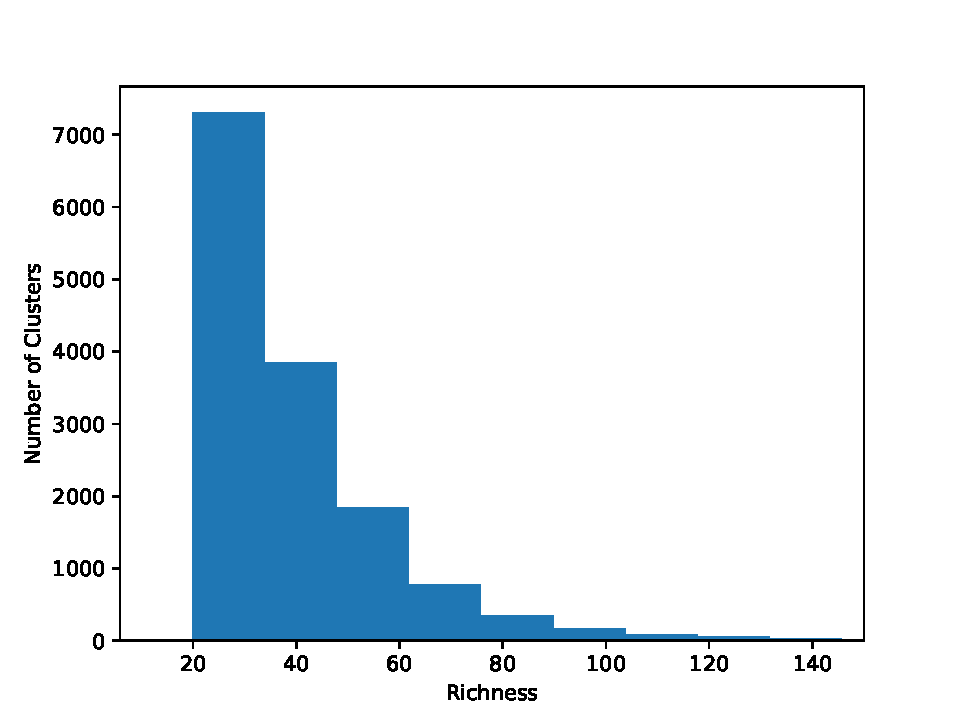
\includegraphics[width=0.5\textwidth]{../redmapper_richness_hist.pdf}
\caption{This plot shows a histogram of the distribution of the richnesses of the clusters in the redMaPPer catalog. Evidently, the vast majority of clusters in the RedMaPPer catalog fall between richnesses of 25 and 100. Note that this plot only includes clusters from RedMaPPer that were used in our analysis and thus does not include clusters that fell outside the range of our maps or were too close to point sources. }
%\label{RedMaPPer Richness Distribution}
\end{figure}

 \chapter{Theory and Methods}
\section{The tSZ Effect}
The tSZ effect is the result of inverse Compton scattering of photons from the CMB off of high energy electrons in hot gas. When CMB photons go through hot cluster gas they gain energy from the high energy electrons. Then when we measure the CMB these photons produce a frequency-dependent change in the observed CMB temperature along the LOS to the galaxy cluster (Greco et al.). The tSZ effect is quantified by the Compton-y parameter. The observationally relevant Compton-y parameter is the Comptonization parameter integrated along the full LOS within some aperture radius,
\begin{equation}
Y^{cyl}_{c}=d^{-2}_A(z) \frac{\sigma_T}{m_e c^2}\int_0^{R_c} 2 \pi R dR \int_{-\inf}^{\inf} dl P_e(r,M,z)
\end{equation}
Where $Y^{cyl}_{c}$ is the observed Compton-y parameter, $d_A(z)$ is the angular diameter distance to the cluster,$\sigma_T$ is the Thomson scattering cross-section, $m_e c^2$ is the rest mass of the electron, R is the  projected radius which we integrate up to $R_c$,  and $P_e(r,M,z)$ is the electron pressure profile (Greco et al.).
\section{Aperture Photometry}
To extract the Compton-y parameter from the CMB maps and differentiate it from effects of the dust, and bulk kSZ, we perform aperture photometry on the CMB maps at the locations of clusters indicated by the cluster catalogs. To perform aperture photometry we define a circular aperture of some radius (which we determined empirically to correspond to the typical radius of the tSZ effect at each frequency) surrounded by an annulus. We then subtract the mean pixel value in the annulus from the circular aperture and define the observed signal, $S_i$, to be the sum of the pixel values inside the circular aperture after this subtraction. The mean value of the annulus is subtracted to correct for large-scale foreground contamination, assuming it is roughly constant over the extracted aperture (Greco et al.). This signal, $S_i$, is then modeled just as described in Greco et al.,
\begin{equation}
\begin{aligned}
S_i=a_i Y^{cyl}_{c}+b_i D_c +\delta T_{CMB} \\
a_i=g(\nu_i) T_{CMB}\\
b_i=\left(\frac{\nu_i(1+z)}{\nu_0}\right)^\beta B (v_i(1+z),T_{dust})\left[\frac{\partial B(\nu_i,T)}{\partial T} \right]^{-1}_{T_{CMB}},
\end{aligned}
\end{equation}


where $g(\nu_i)=h\nu_i/k_B T_{CMB} coth(h\nu_i/2k_B T_{CMB})$, $T_{CMB}=2.7255 K$, $D_c$ is the amplitude of the dust emission integrated along the full LOS within the aperture radius, $v_0=353$ GHz is the reference frequency, $\beta=1.78$ is the dust spectral emissivity index, $T_{dust}= 20 K$ is the dust temperature, $B(\nu_i,T)$ is the Planck function, and $\delta T_{CMB}$ provides a constraint on bulk kSZ.\par 
We do a weighted sum of the aperture photometry values for all the clusters at each frequency in which the weight of each value is inversely proportional to the amount of noise in that area of the map. Then we fit these weighted sums to the model above using emcee.
\par We use a similar methodology to fit for tSZ, dust, and rSZ (rather than bulk kSZ). When fitting for these parameters, we use a slightly different model.
\begin{equation}
\begin{aligned}
S_i=a_i Y^{cyl}_{c}+b_i D_c +Y^{cyl}_{c}g_{rel}(\nu_i,T_{eff}) \\
a_i=g_{rel}(\nu_i,T_{eff}) T_{CMB}\\
b_i=\left(\frac{\nu_i(1+z)}{\nu_0}\right)^\beta B (v_i(1+z),T_{dust})\left[\frac{\partial B(\nu_i,T)}{\partial T} \right]^{-1}_{T_{CMB}},
\end{aligned}
\end{equation}
where $g_{rel}(\nu,T_{eff})$ is $g(\nu)$ modified with relativistic corrections thus introducing a dependency on the effective temperature ($T_{eff}$). In the case $T_{eff}=0$, $g_{rel}(\nu,T_{eff}=g(\nu)$. A plot of $g_{rel}(\nu,T_{eff}$ for different values of $T_{eff}$ and a plot of the dust coefficient are shown below.

\begin{figure}[h]
\centering
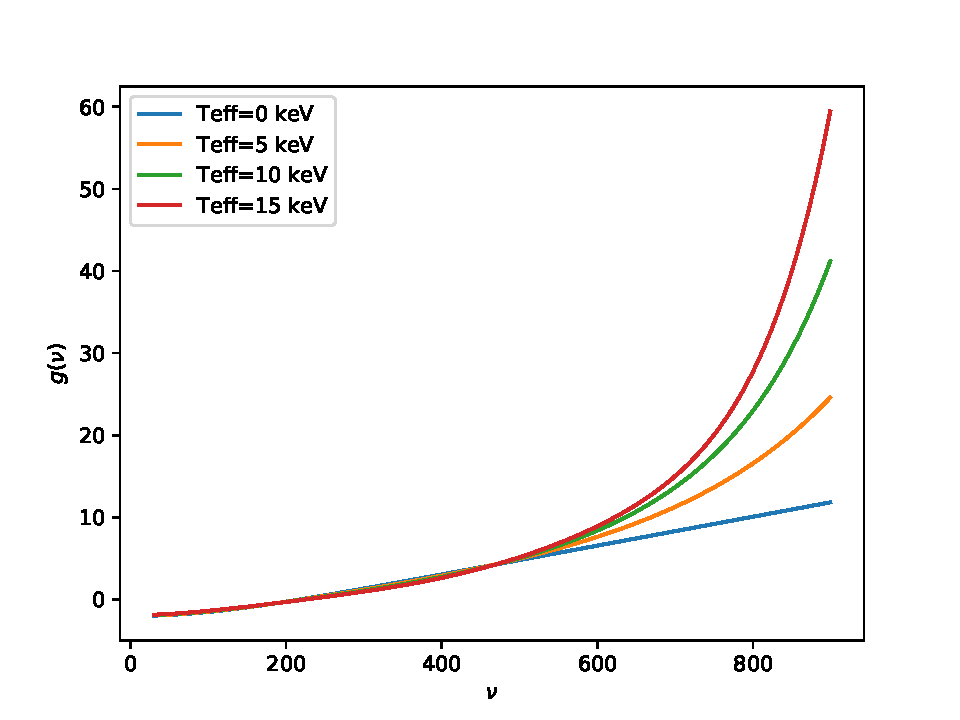
\includegraphics[width=0.5\textwidth]{../gnu.pdf}
\caption{This plot shows $g(\nu)$ as a function of frequency and for different values of $T_{eff}$. }
%\label{$g(\nu)$}
\end{figure}

\begin{figure}[h]
\centering
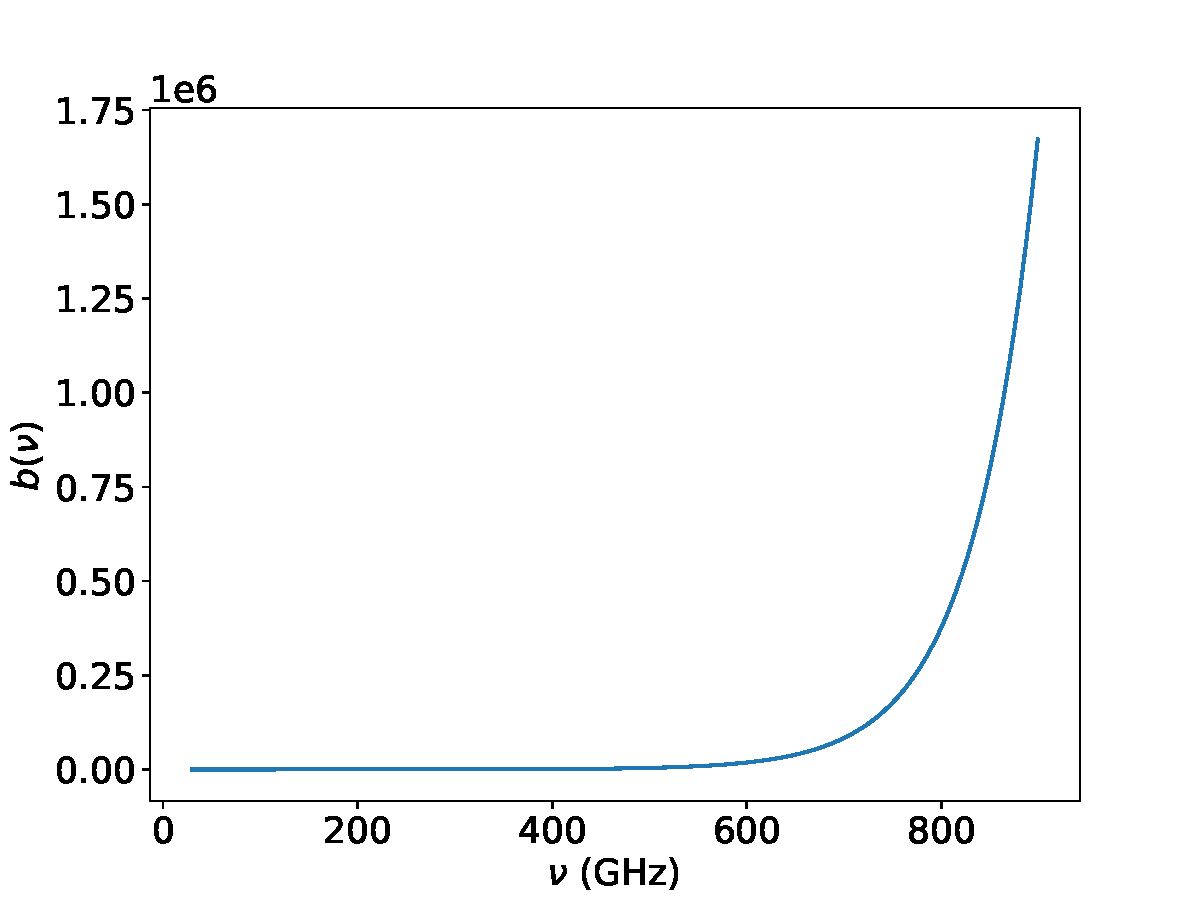
\includegraphics[width=0.5\textwidth]{../bdust.pdf}
\caption{This plot shows the dust coefficient as a function of frequency at a constant value of z=0.36315244, which is the average z value for our sample of galaxy clusters.}
%\label{$g(\nu)$}
\end{figure}


\section{Stacking}
In addition to doing this aperture photometry, we also use rectangular cutouts of the maps centered on the clusters as the to create unweighted and weighted stacks. These stacks provide a visual representation of the SZ effect at the different frequencies. Additionally ,the mean of the aperture photometry values of all the clusters at a given frequency should be the same as the aperture photometry values of the corresponding stacks. Thus, we were able to use the stacks to confirm our aperture photometry methodology. 
\begin{figure}[ht]
  %\centering
 % \textbf{RedMaPPer Stacks}\par\medskip
  \begin{subfigure}[b]{0.5\linewidth}
    \centering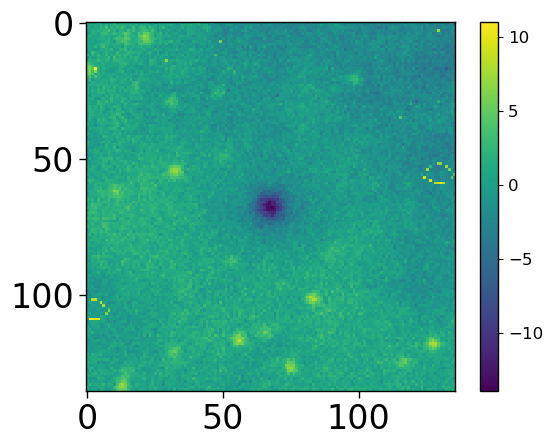
\includegraphics[width=200pt]{../f90_redmapper_wstack.png}
    \caption{\label{fig:fig1}}
  \end{subfigure}
  %\newline
  \begin{subfigure}[b]{0.1\linewidth}
    \centering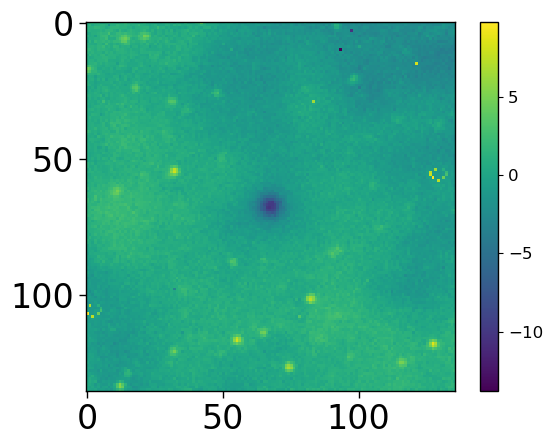
\includegraphics[width=200pt]{../f150_redmapper_wstack.png}
    \caption{\label{fig:fig2}}
  \end{subfigure}
  \newline
  \begin{subfigure}[b]{0.5\linewidth}
    \centering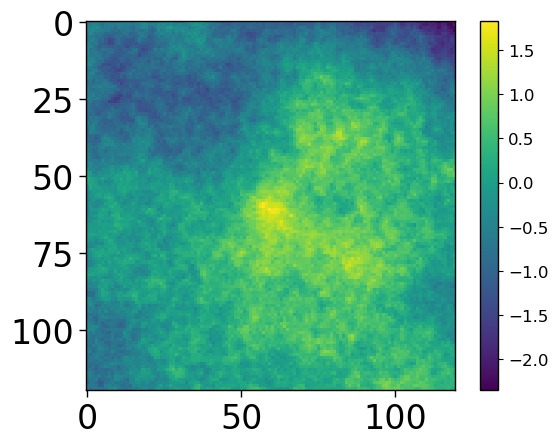
\includegraphics[width=200pt]{../f217_redmapper_wstack.png}
    \caption{\label{fig:fig3}}
  \end{subfigure}
 \begin{subfigure}[b]{0.1\linewidth}
    \centering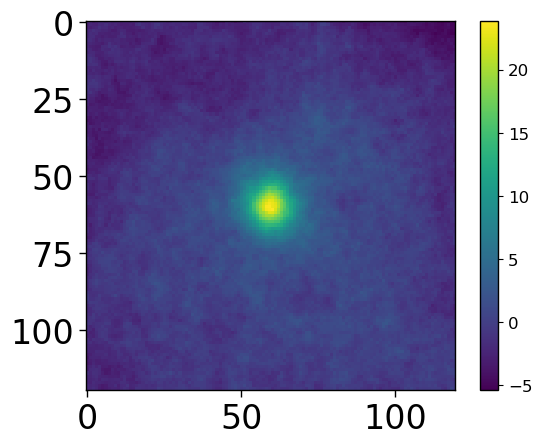
\includegraphics[width=200pt]{../f353_redmapper_wstack.png}
    \caption{\label{fig:fig3}}
  \end{subfigure}
  \newline
 \begin{subfigure}[b]{0.5\linewidth}
    \centering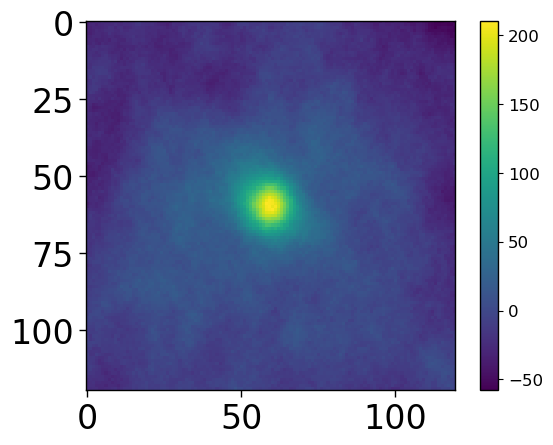
\includegraphics[width=200pt]{../f545_redmapper_wstack.png}
    \caption{\label{fig:fig3}}
  \end{subfigure}
   \begin{subfigure}[b]{0.1\linewidth}
    \centering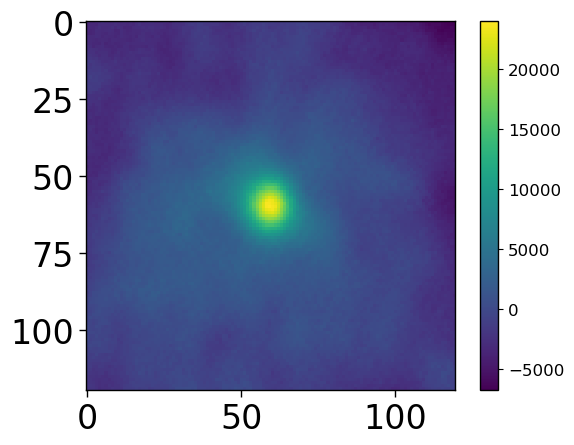
\includegraphics[width=200pt]{../f857_redmapper_wstack.png}
    \caption{\label{fig:fig3}}
  \end{subfigure}
  \caption{This shows the weighted stack stamp plots the RedMaPPer catalog. The 90 GHz and 150 GHz (subfigures a and b respectively) are on the ACT maps while the 217, 353, 545, and 857 GHz maps (subfigures c, d, e, and f respectively) are on the Planck maps. }
\end{figure}
\chapter{Results}
Before doing the mcmc fitting, we performed a linear fit to the data by minimizing chi-squared. Here we only fit for two parameters, the Compton-y parameter and the integrated amplitude of the dust emission. Using this fit we found that $Y^{cyl}_{c}=7.96871772*10^{-17}$ and $D_c=5.74833793*10^{-18}$. This fit is plotted in the figure below. The code we wrote for the linear fit was based on Hogg et al., 2010.

\begin{figure}[h]
\centering
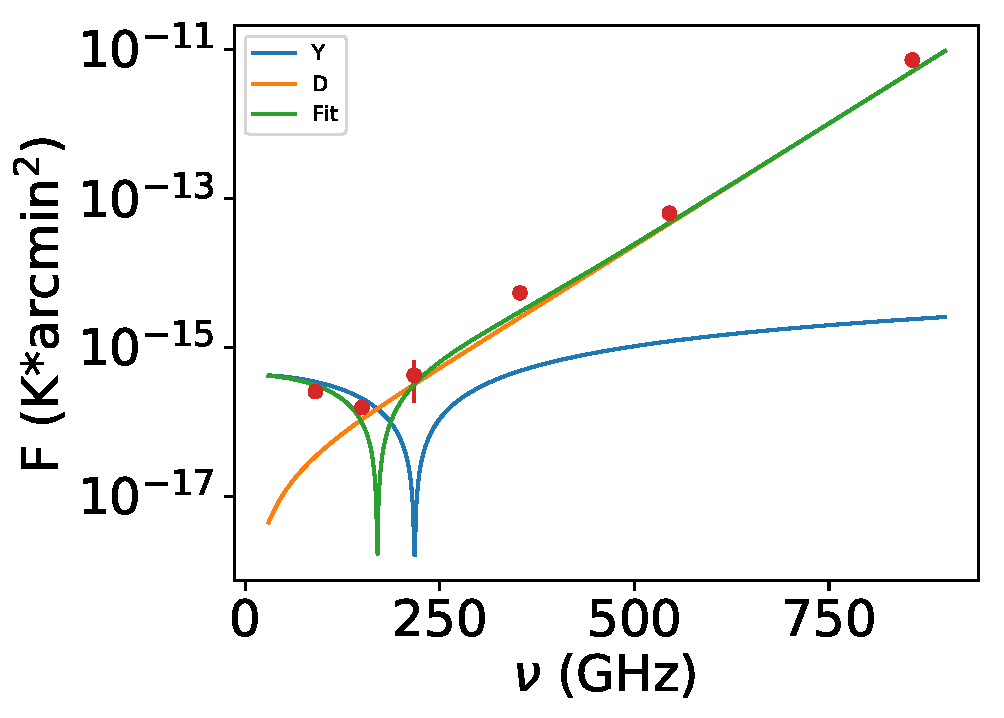
\includegraphics[width=0.5\textwidth]{../redmapper_apfluxes_fitlog.pdf}
\caption{This plot shows a linear fit of the data using only two fit parameters: Y (i.e. the Compton-y parameter) and D (the dust parameter). Note that the y-axis is on a log scale and thus shows the absolute value.}
%\label{$g(\nu)$}
\end{figure}

\par However, the linear fit algorithm was not effective at fitting for bulk kSZ or rSZ (in addition to Compton-y and dust). In order to effectively fit for these parameters we needed to include priors which constrained the possible values of the parameters. Without such priors, the fit algorithm resulted in physically nonsensical values (e.g. $T_{eff}<0$ and bulk kSZ significantly deviating from 0). Thus, we used mcmc to fit with priors. For the mcmc fit with parameters Compton-y, dust, and effective temperature, we found that $Y=6.3e-17^{+2.1e-18}_{-2.3e-18}$, $D=5.7e-18^{+3.3e-19}_{-3.3e-19}$, and $T_{eff}<1.4e8$. For the mcmc fit with parameters Compton-y, dust, and bulk kSZ, we found that $Y=7.9e-17^{+2.1e-18}_{-2.1e-18}$, $D=5.8e-18^{+3.3e-19}_{-3.4e-19}$, and $kSZ<-3.5e-18$. The results of these fits are shown in the plots and table below. The corner plots were generated using code from Foreman-Mackey, 2016. 

\begin{figure}[h]
\centering
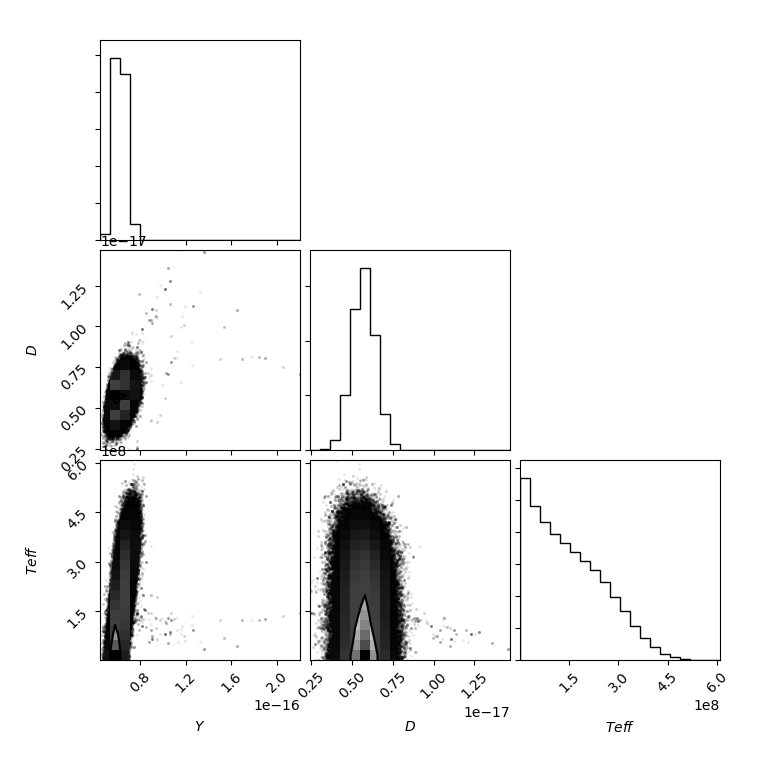
\includegraphics[width=0.5\textwidth]{../CornerTeffplot.png}
\caption{This plot shows the corner plot of the results of the mcmc fit for Compton Y, dust, and the effective temperature. The priors used were $ 1e-17 < Y < 1e-14, 1e-19< D < 1e-16$ and $0.0 < T_{eff} <1e10.$. The resulting best fit parameters were $Y=6.3e-17^{+2.1e-18}_{-2.3e-18}$, $D=5.7e-18^{+3.3e-19}_{-3.3e-19}$, and $T_{eff}<1.4e8$, where the errors on Y and D are 1 sigma and the constraint on $T_{eff}$ is 2 sigma.}
\end{figure}

\begin{figure}[h]
\centering
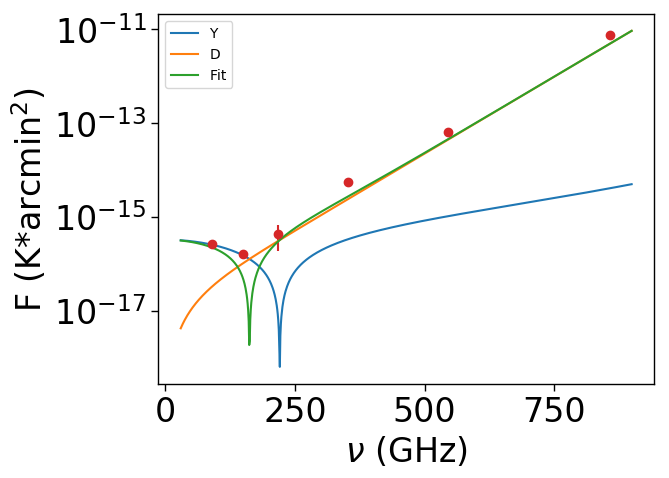
\includegraphics[width=0.5\textwidth]{../redmapper_apfluxes_Tefffitlog.png}
\caption{This plot shows  the results of the mcmc fit for Compton Y, dust, and the effective temperature on a logarithmic y-scale. The priors used were $ 1e-17 < Y < 1e-14, 1e-19< D < 1e-16$ and $0.0 < T_{eff} <1e10.$. The resulting best fit parameters were $Y=6.3e-17^{+2.1e-18}_{-2.3e-18}$, $D=5.7e-18^{+3.3e-19}_{-3.3e-19}$, and $T_{eff}<1.4e8$, where the errors on Y and D are 1 sigma and the constraint on $T_{eff}$ is 2 sigma.}
\end{figure}

\begin{figure}[h]
\centering
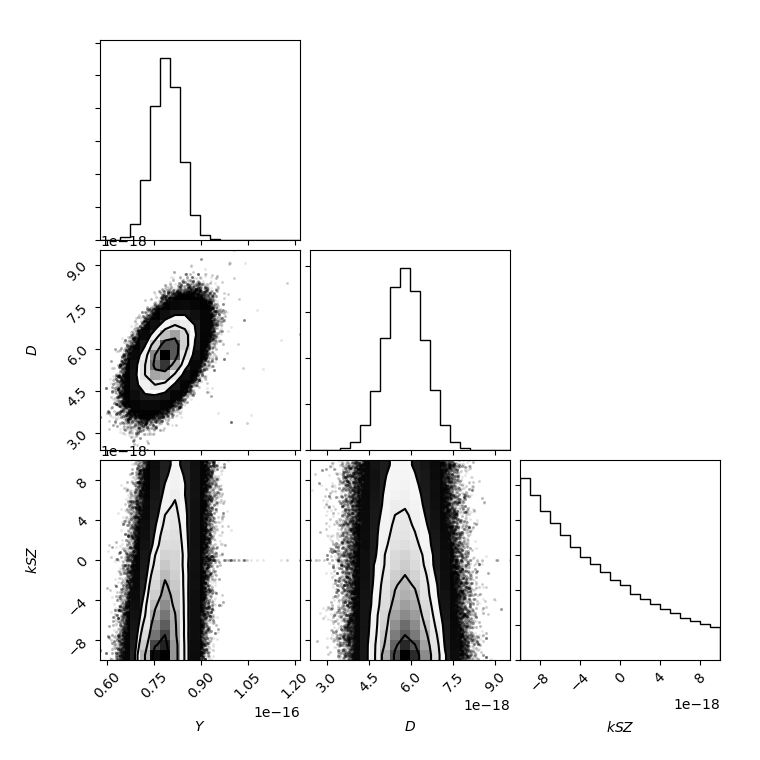
\includegraphics[width=0.5\textwidth]{../BulkkSZplot.png}
\caption{This plot shows the corner plot of the results of the mcmc fit for Compton Y, dust, and the bulk kSZ. The priors used were $ 1e-17 < Y < 1e-14, 1e-19< D < 1e-16$ and $-1e-17 < kSZ <1e-17.$ The resulting best fit parameters were $Y=7.9e-17^{+2.1e-18}_{-2.1e-18}$, $D=5.8e-18^{+3.3e-19}_{-3.4e-19}$, and $kSZ<-3.5e-18$, where the errors on Y and D are 1 sigma and the constraint on kSZ is 2 sigma.}
\end{figure}

\begin{figure}[h]
\centering
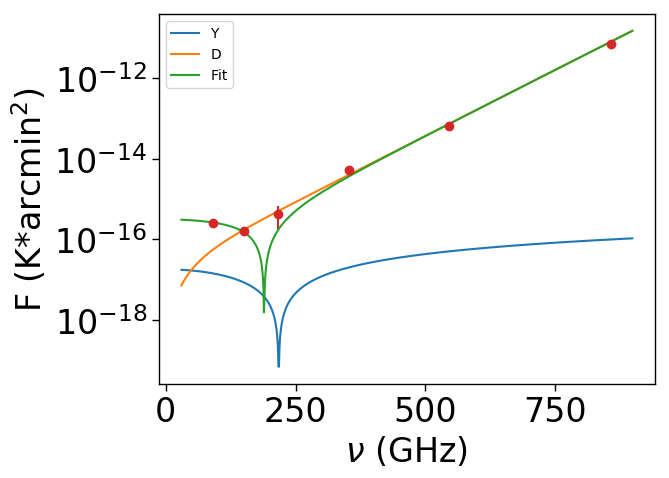
\includegraphics[width=0.5\textwidth]{../redmapper_apfluxes_kSZfitlog.png}
\caption{This plot shows  the results of the mcmc fit for Compton Y, dust, and the bulk kSZ on a logarithmic y-scale. The priors used were $ 1e-17 < Y < 1e-14, 1e-19< D < 1e-16$ and $-1e-17 < kSZ <1e-17.$ The resulting best fit parameters were $Y=7.9e-17^{+2.1e-18}_{-2.1e-18}$, $D=5.8e-18^{+3.3e-19}_{-3.4e-19}$, and $kSZ<-3.5e-18$, where the errors on Y and D are 1 sigma and the constraint on kSZ is 2 sigma.} %not sure the constraint value is correct
\end{figure}

\begin{table}[h!]
\centering
\begin{tabular}{||c c c c||} 
 \hline
Compton-y & Dust & rSZ & kSZ \\ [0.5ex] 
 \hline\hline
 6.3e-17 & 5.7e-18 & <1.4e8 & N/A \\ 
 7.9e-17 & 5.8e-18 & N/A & <-3.5e-18 \\ [1ex] 
 \hline
\end{tabular}
\caption{This table shows the best fit values and constraints of the two fits we performed using the emcee python package. The first row shows the best fit values and constraints for the rSZ fit and the second row shows the best fit values and constraints for the kSZ fit.}
\label{table:1}
\end{table}

\chapter{Discussion and Conclusion}
\par Comparing our results to previous work on this topic, 
\par There are a number of improvements to our analysis that could be made in future work. For example, in our analysis we assumed that each map corresponded to a single frequency. However, this assumption is not entirely accurate. In reality, the CMB maps are not measured at a single, exact frequency, but rather consist of an integrated signal over some frequency bandpass. Thus, our analysis could be enhanced by taking this into account. In future research, we could also account for the beam convolution in the CMB maps.



\chapter{Acknowledgements}
This work would not have been possible without the invaluable assistance of Dr. Mathew Madhavacheril. We would also like to thank Prof. David Spergel,  Dr. Colin Hill, and Dr. Nick Battaglia for providing some helpful insights regarding the direction of this project.   Dr. Colin Hill's code for rSZ was also extremely useful. Finally, we would like to acknowledge Sigurd Naess for providing the ACT coadd maps.

\chapter{References}
A. D. Hincks, R. Genova-Santos, G. Luzzia and E. S. Battistellia. Submitted to JCAP March 8th, \par 2018. \newline
D. W. Hogg, , J. Bovy,  and D. Lang,  2010, ArXiv e-prints, arXiv:1008.4686 \newline
F., De Bernardis et al., J. Cosmol. Astropart. Phys. 03 008 (2017). \newline
Foreman-Mackey, corner.py: Scatterplot matrices in Python, Journal of Open Source Software, 1(2), \par 24, (2016).\newline
J. Erler, K. Basu, J. Chluba, and F. Bertoldi, MNRAS 000, 1?22 (2018).
J. P. Greco, J. C. Hill, D. N. Spergel, and N. Battaglia,
Astrophys. J. 808, 151 (2015). \newline
P. Bull, T. Clifton, and P. G. Ferreira Phys. Rev. D 85, 024002 (2012). \newline
Planck, P. A. R. Ade et al., Astron. Astrophys. 561, A97 (2014), arXiv:1303.5090

\end{document}
